\documentclass[tikz,border=2pt]{standalone}
\usepackage{tikz}
\usetikzlibrary{calc}

\begin{document}
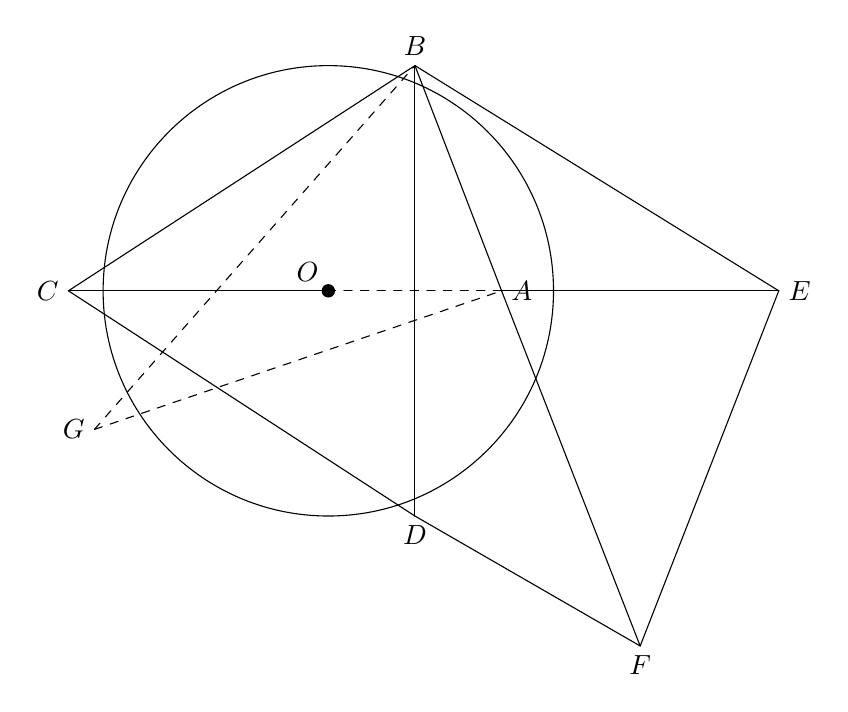
\begin{tikzpicture}[scale=1.1, line cap=round, line join=round]
  % Coordinates
  \coordinate (O) at (0,0);
  \coordinate (A) at (2,0);
  \coordinate (C) at (-3,0);
  \coordinate (B) at (1,2.6);
  \coordinate (D) at (1,-2.6);
  \coordinate (E) at (5.2,0);
  \coordinate (F) at (3.6,-4.1);
  \coordinate (G) at (-2.7,-1.6);

  % Circle
  \draw (O) circle (2.6);

  % Solid segments on the horizontal line, excluding AO
  \draw (C)--(O);
  \draw (A)--(E);

  % AO changed to dashed
  \draw[dashed] (A)--(O);

  % Other solid segments
  \draw (C)--(B);
  \draw (B)--(D);
  \draw (C)--(D);
  \draw (B)--(A);
  \draw (B)--(E);
  \draw (A)--(F);
  \draw (E)--(F);
  \draw (D)--(F);

  % Dashed auxiliary segments
  \draw[dashed] (G)--(B);
  \draw[dashed] (G)--(A);

  % Point O
  \fill (O) circle (2.2pt);

  % Labels
  \node[above] at (B) {$B$};
  \node[below] at (D) {$D$};
  \node[right] at (A) {$A$};
  \node[left] at (C) {$C$};
  \node[right] at (E) {$E$};
  \node[below] at (F) {$F$};
  \node[left] at (G) {$G$};
  \node[above left] at (O) {$O$};
\end{tikzpicture}
\end{document}
